\section{Graphs}\label{sec:graphs}

\begin{definition}\leavevmode
\begin{enumerate}
    \item \label{def:graph} A \textbf{graph} $G=(V, E)$ is a pair of sets $V=V(G)$ and $E=E(G)$, where $V$ is a non-empty set and $E$ is a (possibly empty) set consisting only of two-element sets of the form $\{a, b\}$, where $a \in V$ and $b \in V$.  The set $V(G)$ is called the set of \textbf{vertices} of $G$ and the set $E(G)$ is called the set of \textbf{edges} of $G$.
    \item The number of vertices in a graph is denoted by $v=v(G)=|V(G)|$ and the number of edges in a graph is denoted by $e=e(G)=|E(G)|$.  It is possible that $v=\infty$ or $e=\infty$, meaning that there is no such (finite) number.
    \item If $\gamma=(v_1, v_2)\in E$, then we say that $\gamma$ \textbf{connects} $v_1$ and $v_2$ and that $v_1$ and $v_2$ are \textbf{adjacent}.
    \item \label{def:graph_diagram} Let $D$ be a subset of a space (typically the Euclidean Plane, $\mathbb{R}^2$) consisting of points and arcs connecting those points, such that the arcs only meet the points in their boundaries.  Given a graph $G$, $D$ is said to be a \textbf{graph diagram} for $G$ if:
    \begin{enumerate}
        \item the vertices of $G$ are in one-to-one correspondance with the points of $D$, and
        \item the edges of $G$ are in one-to-one correspondance with the arcs of $D$.
    Note that a graph diagram $D$ is sometimes referred to as an \textbf{embedding}, particularly if the space is not $\mathbb{R}^2$.  We will often not distinguish between a graph and its projection unless it is important to do so. (For example, we may say ``draw a graph that...'' which clearly means ``draw a projection of a graph in $\mathbb{R}^2$ such that...''.)
    \end{enumerate}

    \item Two graphs are \textbf{equal} if they have equal vertex and edge sets.  Two graph diagrams are equal if they represent equal graphs.
\end{enumerate}
\end{definition}

Another name for vertex is \textit{node}, and another name for an edge is a \textit{link}.

\begin{lemma} \label{lem:simple_graph}Let $G$ be a graph.  Then $G$ has no \textit{loops, i.e.} edges connecting a vertex to itself, and $G$ has no \textit{skeins, i.e.} collections of more than one edge connecting a pair of vertices.
\end{lemma}

\begin{remark} In other formulations of Graph Theory, using multisets one can define graphs that have loops and skeins, and then one would create a definition of a graph without these, typically called \textit{simple graphs}.  In this other formulation, Lemma \ref{lem:simple_graph} shows that we will restrict our discussion to simple graphs.

Often, one may consider graphs whose edges have a direction to them, \textit{i.e.} whose edges are ordered pairs, rather than sets, which has huge ramifications when formulating a notion of paths (see Chapter \ref{sec:euler}).  We will not study these types of graphs either, called \textit{directed graphs}, but they are nonetheless a very important concept in Graph Theory.
\end{remark}

\begin{examples} Let $v$ be a natural number.  Draw several examples of each of the following graphs.
    \begin{enumerate}
        \item The \textbf{null graph} is a graph with $E=\emptyset$.
        \item The \textbf{cyclic graph} $C_v$ consists of $v$ vertices $v_1, v_2, \ldots, v_v$ and edges of the form $\{v_i, v_{i+1}\}$ for all $i$ with $1\leq i \leq v$ along with $\{v_v, v_1\}$.
        \item The \textbf{complete graph} on $v$ vertices, $K_v$, is the graph consisting of $v$ vertices and all possible edges between them.
    \end{enumerate}
\end{examples}

\begin{theorem} \label{thm:edges_in_Kv} Let $K_v$ denote the complete graph on $v$ vertices.  Then $e=|E(K_v)|= \frac{1}{2} v \cdot (v-1)$.
\end{theorem}

\begin{definition}
    Suppose $G$ and $H$ are graphs such that $V(H) \subseteq V(G)$ and $E(H) \subseteq E(G)$.  Then $H$ is a \textbf{subgraph} of $G$, and $G$ is a \textbf{supergraph} of $H$.
\end{definition}

\begin{example} Given any graph $G$ and any subset $X$ of $V(G)$, the \textbf{induced subgraph} of $G$ by $X$ is the subgraph whose vertex set is $X$ and whose edge set is all the edges of $G$ whose vertices both lie in $X$.  Draw an example of a graph with 7 vertices and 10 edges, and draw three different induced subgraphs.
\end{example}

\begin{lemma} Every graph $G$ is the subgraph of a complete graph, denoted $K_{v(G)}$.
\end{lemma}

\begin{definition} Let $G$ and $H$ be graphs.
    \begin{enumerate}
    \item The \textbf{complement} of $G$, denoted $\overline{G}$, is the graph given by:
    \begin{itemize}
        \item $V(\overline{G}) = V(G)$, and
        \item $E(\overline{G}) = K_{v(G)} \setminus E(G)$.  That is, the edges of $\overline{G}$ are precisely the edges ``missing'' from $G$ to make up $K_{v(G)}$.
    \end{itemize}

    \item Suppose there are a pair of bijections $C_V$ and $C_E$ between the vertex and edges sets of $G$ and $H$, respectively, which \textit{respect one another} in the following way: if the edge $\{v_1, v_2\}\subseteq E(G)$ is paired under $C_E$ to an edge $\{w_1, w_2\}\subseteq E(H)$, then without loss of generality the vertices $v_1$ and $w_1$ are paired and the vertices $v_2$ and $w_2$ are paired under $C_V$.  Then the pair $(C_V, C_E)$ is called an \textbf{isomorphism} between $G$ and $H$, and $G$ and $H$ are said to be \textbf{isomorphic}, written $G \cong H$.
\end{enumerate}
\end{definition}

\begin{theorem}[Isomorphism is an equivalence relation]  Let $G$, $H$, and $K$ be graphs.
\begin{enumerate}
    \item (Reflexivity) $G$ is isomorphic to $G$.
    \item (Symmetry) If $G$ is isomorphic to $H$, then $H$ is isomorphic to $G$.
    \item (Transitivity) If $G$ is isomorphic to $H$ and $H$ is isomorphic to $K$, then $G$ is isomorphic to $K$.
\end{enumerate}
\end{theorem}

\begin{corollary} If $G$ and $H$ are isomorphic graphs, then $v(G)=v(H)$ and $e(G)=e(H)$.
\end{corollary}

\begin{definition} Let $G$ be a graph and $a\in V$ be a vertex.
\begin{enumerate}
    \item The \textbf{degree} of $a$, $\deg(a)$, is the number of edges containing $a$ as one of its vertices.  (This is sometimes called the \textbf{valence}).  Vertices may be called \textbf{even} or \textbf{odd} if they have even or odd degreee, respectively.
    \item If $G$ is a graph such that every vertex has the same degree, say $r$, then $G$ is said to be \textbf{regular of degree} $r$.
    \item The \textbf{degree sequence} of $G$ is the ordered $v$-tuple of nonincreasing degrees of the vertices of $G$.  That is, suppose that the vertices of $G$ are $v_1, v_2, \ldots, v_v$, and the ordering of them has been choosen such that $\deg(v_i)\geq \deg(v_{i+1})$ for all $i$ with $1 \leq i \leq v$.  Then the degree sequence of $G$ is an ordered list $(\deg(v_1), \deg(v_2), \ldots, \deg(v_v))$.
\end{enumerate}
\end{definition}

\begin{remark} As in the definition of ordered pair (Definition \ref{def:bijection}), an ordered $n$-tuple, for $n$ some natural number, is an ordered list where repetition is possible.  The word ``tuple'' is a generalization of the word ``pair''. Similarly to an ordered pair, one may form a definition of an ordered pair using sets for absolute clarity, such as for a 4-tuple: $$(1,2,3,3) = \{\{1\}, \{1,2\}, \{1,2,3\}, \{1,2,3,4\}\}.$$
Two ordered $n$-tuples are the same if they contain the same items in the same order.
\end{remark}

\begin{theorem}\label{thm:degree_seq_invt} If $G$ and $H$ are isomorphic graphs, then their degree sequences are equal.
\end{theorem}

\begin{example} \label{ex:non-iso_graphs} Show that the two graphs drawn in Figure \ref{fig:non-iso_graphs} are not isomorphic.
\end{example}
\begin{figure}[hb]
\begin{center}
    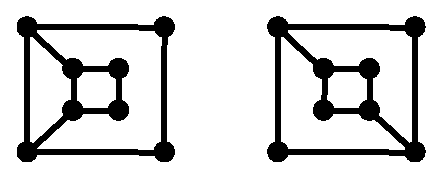
\includegraphics[width=.5\textwidth]{non_iso_graphs.eps}
    \label{fig:non-iso_graphs}
    \caption{Two non-isomorphic graphs}
\end{center}
\end{figure}

\begin{exercises}
\begin{enumerate}
    \item Let $v$ be a natural number.  The \textbf{wheel graph} on $v$ vertices, denoted $W_v$, is the graph obtained from $C_{v-1}$ by adding a new ``complete'' vertex, \textit{i.e.} a vertex that is adjacent to every other vertex.  Draw some examples of wheel graphs, then determine and prove the correctness of a formula for the number of edges in $W_v$.
    \item Let $G$ be a graph.  Determine and prove correctness of a formula for the number of edges in $\overline{G}$ given only $v(G)$ and $e(G)$.
    \item Determine all numbers $v$ such that $C_v \cong K_v$. Prove your claim.
    \item The degree sequence is what is called an \textbf{isomorphism invariant} meaning that if $G \cong H$, then the degree sequence of $G$ equals the degree sequence of $H$ (by Theorem \ref{thm:degree_seq_invt}).  State the contrapositive of this statement, and find a pair of graphs with the same number over vertices (at least 5), edges (at least 7), yet a different degree sequence.  What can you conclude about these graphs?  Find a pair of non-isomorphic graphs with at least 5 vertices, none of degree 2, for which their degree sequences do not prove their non-isomorphic status.  This shows that the degree sequence is not a \textit{complete} invariant.
    \item Prove that $C_v \cong \overline{C_v}$ if and only if $v = 5$.
    \item Prove that if $G \cong \overline{G}$, then $v$ or $v-1$ is divisible by 4.
    \item Prove that if $G_1 \cong G_2$ and $A_1 \subseteq G_1$ then there exists a subgraph $A_2 \subseteq G_2$ with $A_1 \cong A_2$.  Use this to reprove the non-isomorphism of Example \ref{ex:non-iso_graphs}.
    \item Classify all graphs with 3 vertices up to isomorphism.  That is, find a list of pairwise non-isomorphic graphs such that any graph with 3 vertices is isomorphic to exactly one of the graphs in your list.
    \item Prove that $G_1 \cong G_2$ if and only if $\overline{G_1} \cong \overline{G_2}$.
    \item A \textit{partition} of a set is a decomposition into non-intersecting sets.  That is, $\{1,2,3\} = \{1,2\} \cup \{3\}$ is a partition, but $\{1,2,3\} = \{1,2\} \cup \{2, 3\}$, which is a true statement, is not a partition.

    Let $G$ be a graph such that $V(G)$ can be partitioned into two sets $A$ and $B$ with the property that no edges of $G$ have both vertices in $A$ or both vertices in $B$.  Then $G$ is called a \textbf{bipartite graph}.

    One family of examples of bipartite graphs are the \textbf{complete bipartite graphs}, $K_{m,n}$: given natural numbers $m$ and $n$, the complete bipartite graph on $m$ and $n$ vertices is a bipartite graph with partition $A\cup B$, where $|A| = m$ and $|B| = n$, and all possible edges.  Draw some examples of complete bipartite graphs.

    Let $m$, $n$, $a$, and $b$ be natural numbers. Prove that $K_{m,n} \cong K_{a,b}$ if and only if $m = a$ and $n = b$.

    \item Create formulae (and prove their correctness) for the number of edges of each of the following families of graphs, based on the number of vertices ($v$):
    \begin{itemize}
        \item $K_v$
        \item $C_v$
        \item $\overline{C}_v$
        \item $W_v$ (wheel graph)
        \item $K_{m,n}$.
    \end{itemize}

    \item Prove that a graph with $v \geq 2$ has two vertices with the same degree.

\end{enumerate}
\end{exercises}
